\documentclass[12pt]{article}
\usepackage{amsmath}
\usepackage{amsthm}
\usepackage{graphicx,psfrag,epsf}
\usepackage{enumerate}
\usepackage{natbib}
\usepackage{url} % not crucial - just used below for the URL 
\usepackage{algorithm}
\usepackage{algpseudocode}
\usepackage{subfig}
\usepackage{authblk}
\usepackage{verbatim} %used to comment out unnecessary contents

%\pdfminorversion=4
% NOTE: To produce blinded version, replace "0" with "1" below.
\newcommand{\blind}{0}

% DON'T change margins - should be 1 inch all around.
\addtolength{\oddsidemargin}{-.5in}%
\addtolength{\evensidemargin}{-.5in}%
\addtolength{\textwidth}{1in}%
\addtolength{\textheight}{-.3in}%
\addtolength{\topmargin}{-.8in}%

%environment
\newtheorem{thm}{Theorem}
\newtheorem{lem}{Lemma}
\newtheorem{cor}{Corollary}
\newtheorem*{defi*}{Properties}
\newtheorem{asn}{Assumption}
\newcommand*\mean[1]{\bar{#1}}
%\newproof{proof}{Proof}
%\newproof{proof}{Proof}
\begin{document}

\def\spacingset#1{\renewcommand{\baselinestretch}%
{#1}\small\normalsize} \spacingset{1}

\title{\bf Local Distance Correlation}
\author[1]{Cencheng Shen\thanks{cshen@temple.edu}}
\author[2]{Joshua T. Vogelstein\thanks{jovo@jhu.edu}}
\author[3]{Carey E. Priebe\thanks{cep@jhu.edu}}
\affil[1]{Department of Statistics, Temple University}
\affil[2]{Department of Biomedical Engineering and Institute of Computational Medicine, Johns Hopkins University}
\affil[3]{Department of Applied Mathematics and Statistics, Johns Hopkins University}
\maketitle

\bigskip
\begin{abstract}
In this paper we propose a local distance statistic to test independence between data sets. Based on the framework of distance correlation and the idea of k-nearest-neighbor, we construct an advanced test statistic that is not only consistent for testing independence, but also more robust for dealing with data sets of small sample size, high-dimensionality, non-linearity, and noise. The proposed method is easy to use yet achieves excellent performance on a comprehensive simulation setting and real data experiment.
\end{abstract}

\noindent%
{\it Keywords: distance correlation, k-nearest-neighbor, independence test, permutation test}  
\vfill

\newpage
\spacingset{1.45} % DON'T change the spacing!

\section{Introduction}
With the increasing type, size, and dimension of modern data sets, detecting dependency among multiple data sets is one of the most important and fundamental tasks in the big data age. The Pearson correlation coefficient, RV coefficient, the Mantel test, and mutual information (see in \cite{JosseHolmes2013}, \cite{RobertEscoufier1976}, \cite{Mantel1967}) have been the traditional tools for this task, but each has its limitations when dealing with the increasingly complex modern data sets, e.g., the Pearson correlation coefficient, RV coefficient and the Mantel test are mostly useful for finding linear relationship and may be zero for nonlinear dependent data sets, while mutual information requires estimating the probability distribution. 

Many recent methods have been proposed to identify the existence of potential relationships between data sets, among many include \cite{TaskinenOjaRandles2005}, \cite{GrettonEtAl2005}, \cite{SzekelyRizzoBakirov2007}, \cite{GrettonGyorfi2010}, \cite{Reshef2011}, \cite{HellerGorfine2013}, \cite{Reimherr2013}, \cite{SzekelyRizzo2013a}, etc. In particular, the distance correlation method from \cite{SzekelyRizzoBakirov2007} has gained much popularity in the statistical community, due to its theoretical soundness and good numerical performance in testing independence; a similar method from the machine learning point of view is the kernel-based independence test, which is developed in \cite{GrettonEtAl2005}, \cite{GrettonGyorfi2010}, \cite{GrettonEtAl2012}, and connected to the distance-based method in \cite{SejdinovicEtAl2013}.

Despite of current progress in the area, it remains a difficult problem to test dependency on real data; and even the best method in theory may suffer from one or more real challenges underlying the data, such as small sample size, high dimensionality, non-linearity, noise, etc. For example, although distance correlation is consistent against all alternatives for testing independence on Euclidean data, the sample distance correlation under-performs in many high-dimensional or non-linear dependencies for finite-sample testing; the modified distance correlation from \cite{SzekelyRizzo2013a} adjusts the high-dimensional bias, but is still sub-optimal for non-linear dependencies; in comparison, the HHG statistic developed in \cite{HellerGorfine2013} performs much better for testing on non-linear data of small sample size, but it may lose some testing power for linear and high-dimensional dependency.

In this paper we propose a local distance correlation, in order to better address those challenges from modern data analysis. The local test statistic naturally inherits the advantages of the global distance correlation, such as being consistent and can be robust in high-dimensional dependency when applied to the modified distance correlation; and the local method significantly improves the finite-sample testing power of the global version, for testing on data sets of non-linearity, noise, and/or small sample size. Those advantages make our new test statistic the best method thus far, for detecting dependency on real data and complex dependencies. Indeed in our comprehensive simulation setting, local distance correlation is able to achieve a superior performance comparing to the global distance correlation and HHG; and in the real data experiment, the local test statistic also returns the lowest p-value for testing dependency between human brain and human characteristics.

The paper is organized as follows: Section~\ref{main1} reviews the original distance correlation and the modified distance correlation. In Section~\ref{main2} we formulate the local distance correlation for both the original distance correlation and the modified distance correlation. Section~\ref{main3} discusses the evaluation procedure of testing independence, and in Section~\ref{main4} we show some theoretical advantages of local distance correlation. The simulation results are shown in Section~\ref{numer1} to demonstrate the numerical advantages of the local test statistic in various simulated relationships, and Section~\ref{numer2} illustrates its performance on real data sets. We conclude the paper in Section~\ref{conclu}, with proofs, additional propositions, and detailed simulation settings included in the appendix. The Matlab/R code for our method and the simulation is available on github\footnote{\url{https://github.com/jovo/RankdCorr/}}. 

\section{Distance Correlation}
\label{main}
\subsection{Global Distance Correlation}
\label{main1}
Suppose we are given two data sets $\mathcal{X}=[X_{1},\cdots, X_{n}] \in \mathcal{R}^{m_{X} \times n}$ and $\mathcal{Y}=[Y_{1},\cdots, Y_{n}] \in \mathcal{R}^{m_{Y} \times n}$, where $n$ is the sample size, $m_{X}$ and $m_{Y}$ are the dimensions for each data set. Under the classical hypothesis testing framework, we assume that $X_{i}, i=1,\ldots,n$ are identically independently distributed (i.i.d.) as $X$, similarly $Y_{i} \stackrel{i.i.d.}{\sim} Y$. Throughout the paper, we always assume that $X$ and $Y$ have finite second moments, which is a necessary assumption to guarantee the consistency of distance correlation.

For testing independence between $X$ and $Y$, the null and the alternative hypothesis are
\begin{align*}
& H_{0}: X \mbox{ is independent of } Y, i.e., f_{XY}=f_{X}f_{Y},\\
& H_{A}: f_{XY} \neq f_{X}f_{Y},
\end{align*}
where $f_{XY}$ denotes the joint distribution of $(X,Y) \in \mathcal{R}^{m_{X}+m_{Y}}$, and $f_{X}$ and $f_{Y}$ are the marginal distributions. 

To test independence by distance correlation on sample data, we first calculate two Euclidean distance matrices $A, B \in \mathcal{R}^{n \times n}$ for $\mathcal{X}$ and $\mathcal{Y}$ respectively, i.e., $A_{ij}=\|X_{i}-X_{j}\|_{2}$. The sample distance covariance is defined as
\begin{equation}
\label{dCovEqu}
dCov_{n}(\mathcal{X},\mathcal{Y})=\frac{1}{n^2}\sum_{i,j=1}^{n}A^{H}_{ij}B^{H}_{ij},
\end{equation}
where $A^{H}=HAH$, $B^{H}=HBH$ with $H=I_{n}-\frac{J_{n}}{n}$. Then the sample distance variance is defined as
\begin{align*}
dVar_{n}(\mathcal{X}) &=\frac{1}{n^2}\sum_{i,j=1}^{n}A^{H}_{ij}A^{H}_{ij}\\
dVar_{n}(\mathcal{Y}) &=\frac{1}{n^2}\sum_{i,j=1}^{n}B^{H}_{ij}B^{H}_{ij}.
\end{align*}
The squared sample distance correlation is obtained by normalizing the distance covariance
\begin{equation}
\label{dCorrEqu}
dCorr_{n}(\mathcal{X},\mathcal{Y})=\frac{dCov_{n}(\mathcal{X},\mathcal{Y})}{\sqrt{dVar_{n}(\mathcal{X}) \cdot dVar_{n}(\mathcal{Y})}},
\end{equation}
where all of $dCov_{n}, dVar_{n}, dCorr_{n}$ are always non-negative. Note that the $dCor_{n}/dCorr_{n}$ above is actually the square of distance covariance/correlation in \cite{SzekelyRizzoBakirov2007}; but for simplicity we drop the square in the name throughout this paper.

It is shown in \cite{SzekelyRizzoBakirov2007} that as $n \rightarrow \infty$, $dCorr_{n}(\mathcal{X},\mathcal{Y}) \rightarrow dCorr(X,Y) \geq 0$, where $dCorr(X,Y)$ is the population distance correlation of $X$ and $Y$ defined by their characteristic functions. The population distance correlation is $0$ if and only if $X$ and $Y$ are independent, so that the sample distance correlation is a consistent test for independence, i.e., the testing power converges to $1$ as $n$ increases, at any fixed type $1$ error level. Note that in this paper distance correlation always means the sample statistic rather than the population statistic, unless otherwise mentioned.

However, in case of high-dimensional data where the dimension $m_{X}$ or $m_{Y}$ increases with the sample size $n$, the original distance correlation $dCorr_{n}$ is no longer appropriate. For example, even for independent Gaussian distribution, $dCorr_{n} \rightarrow 1$ as $m_{X}, m_{Y} \rightarrow \infty$, such that it is no longer a consistent test in high dimension. This problem is solved by the modified distance correlation proposed in \cite{SzekelyRizzo2013a}:
\begin{equation}
\label{mdCovEqu}
mdCov_{n}(\mathcal{X},\mathcal{Y})=\frac{1}{n(n-3)}(\sum_{i,j=1}^{n}A^{H*}_{ij}B^{H*}_{ij}-\frac{n}{n-2}\sum_{i=1}^{n}A^{H*}_{ii}B^{H*}_{ii}),
\end{equation}
where $A^{H*}_{ij}$ adjusts the entries of $A^{H}$ by
\[A^{H*}_{ij} = \left\{
  \begin{array}{lr}
    \frac{n}{n-1}(A^{H}_{ij}-\frac{A_{ij}}{n}), & \mbox{ if } i \neq j \\
    \frac{n}{n-1}(\frac{\sum_{i}A_{ij}}{n}-\frac{\sum_{i,j}A_{ij}}{n^2}), &\mbox{ if } i = j
  \end{array}
\right.
\] and similarly for $B^{H*}_{ij}$. Then $mdVar_{n}(\mathcal{X})$ can be defined by replacing all $B^{H*}_{ij}$ in Equation~\ref{mdCovEqu} by $A^{H*}_{ij}$, similarly define $mdVar_{n}(\mathcal{Y})$. 

If $mdVar_{n}(\mathcal{X}) \cdot mdVar_{n}(\mathcal{Y}) \leq 0$, the modified distance correlation is set to $0$; otherwise it is defined as
\begin{equation}
\label{mdCorrEqu}
mdCorr_{n}(\mathcal{X},\mathcal{Y})=\frac{mdCov_{n}(\mathcal{X},\mathcal{Y})}{\sqrt{mdVar_{n}(\mathcal{X}) \cdot mdVar_{n}(\mathcal{Y})}}.
\end{equation}
It is shown in \cite{SzekelyRizzo2013a} that $mdCorr_{n}(\mathcal{X},\mathcal{Y}) \rightarrow dCorr(X,Y) \geq 0$, and is an unbiased estimator of the population distance correlation $dCorr(X,Y)$; furthermore, $mdCorr_{n}$ is approximately normal even if $m_{X},m_{Y} \rightarrow \infty$. Thus it is a consistent test of independence for high-dimension data.

To summarize this subsection, both the distance correlation and modified distance correlation are great for testing independence of Euclidean data due to their theoretical consistency, with the modified test statistic being more robust against high-dimensionality. Indeed it is a flourishing concept by a series of papers \cite{BakirovRizzoSzekely2006}, \cite{SzekelyRizzoBakirov2007}, \cite{SzekelyRizzo2009}, \cite{BickelXu2009}, \cite{Kosorok2009}, \cite{Remillard2009}, \cite{LiZhongZhu2012}, \cite{SzekelyRizzo2013a}, \cite{SzekelyRizzo2013b}, \cite{SzekelyRizzo2014}; and the test statistic is not limited to the Euclidean metric as shown in \cite{Lyons2013}. 

However, the required sample size for achieving a good testing power very much depends on the type of dependency underlying the given data, e.g. for perfect linear relationship, sample distance correlation usually requires less than $10$ points for a permutation test to declare significance; but for some nonlinear relationships like circle, sample distance correlation yields no significance even at $n=100$. Because real data rarely exhibits perfect linear relationship, and in practice large amount of data may not always be available, a better finite-sample method is of tremendous value: it not only yields a better testing power for the same sample size, but may also requires much less sample data for the permutation test to declare significance, which in turn saves the running time and data collection process. 

There exists another distance-based method that is consistent and works particularly well for nonlinear dependencies, which is called the HHG statistics in \cite{HellerGorfine2013}. It applies Pearson's chi-square test to ranks of distances within each column rather than directly summing up the products of distances, and is shown to be better than distance correlation and other methods for finite-sample testing of many common nonlinear relationships in \cite{GorfineHellerHeller2012} and \cite{HellerGorfine2013}. However, in our numerical simulations HHG seems to fall a bit short when testing against high-dimensional or close to linear dependency, but is otherwise a strong competitor of the global distance correlation. 

The other method we use as the benchmark in the numerical section is the Mantel test, which simply applies Pearson's correlation to the distance matrices, see in \cite{Mantel1967}. Despite its lack of theoretical guarantee (for example, unlike distance correlation and HHG, it is not consistent against all alternatives), it has been a very popular method so far and commonly used in biology and ecology. In our numerical simulations we will observe that the Mantel test is not consistent for many nonlinear dependencies, and is sub-optimal in almost all types of dependency we consider.

Since there has not been a method that perform well against all possible alternatives in finite-sample testing, it motivates us to propose a local distance correlation that is concurrently robust against small sample size, high-dimensionality, linearity or non-linearity in the following subsection.

\subsection{Local Distance Correlation}
\label{main2}
In this subsection we define the local distance correlation, which is based on k-nearest-neighbor and applicable to both the original distance correlation and the modified distance correlation. From now on, we distinguish the local test statistic as either the local original distance correlation or the local modified distance correlation when they have different behaviors in the context, otherwise we call both as local/global distance correlation since they often share the same properties.

Under the same setting and notation as the global distance correlation in Section~\ref{main1}, we further sort the distance matrix $A$ within column and denote the ranks as $r(A_{ij})$: for each $i=1, \ldots, n$, we always set $r(A_{ii})=0$; then set $r(A_{ij})=k$ if and only if $A_{ij}$ is the $k$th smallest distance in $\{A_{ij}, i=1,\ldots,n\ \& \ i \neq j\}$; break ties deterministically. Similarly sort the distance matrix $B$ within column and denote the ranks by $r(B_{ij})$.

Then we define the local original distance covariance for each $k,l=1,\ldots,n$ as
\begin{equation}
\label{localdCovEqu}
dCov_{kl}(\mathcal{X},\mathcal{Y})=\frac{1}{n^2}\sum_{i,j=1}^{n}A^{H}_{ij}B^{H}_{ij}I(r(A_{ij})<k)I(r(B_{ij})<l),
\end{equation}
and define the local original distance variance as
\begin{align*}
dVar_{k}(\mathcal{X}) &=\frac{1}{n^2}\sum_{i,j=1}^{n}A^{H}_{ij}A^{H}_{ij}I(r(A_{ij})<k)\\
dVar_{l}(\mathcal{Y}) &=\frac{1}{n^2}\sum_{i,j=1}^{n}B^{H}_{ij}B^{H}_{ij}I(r(B_{ij})<l),
\end{align*}
where $I(\cdot)$ is the indicator function. Normalizing local original distance covariance at each $k,l$ yields our local original distance correlation:
\begin{equation}
\label{localdCorrEqu}
dCorr_{kl}(\mathcal{X},\mathcal{Y})=\frac{dCov_{kl}(\mathcal{X},\mathcal{Y})}{\sqrt{dVar_{k}(\mathcal{X}) \cdot dVar_{l}(\mathcal{Y})}}.
\end{equation}
When $k=l$, we simplify the notations to $dCov_{k}$ and $dCorr_{k}$. Note that our local distance correlation refers to the family of test statistics $\{dCorr_{kl}, k,l=1,\ldots,n\}$ rather than each individual $dCorr_{kl}$, i.e., the p-value of local distance correlation equals the smallest p-value among the family, and the testing power of local distance correlation equals the maximal power among the family.

In the same manner, we can define the local modified distance covariance as 
\begin{equation}
\label{localmdCovEqu}
mdCov_{kl}(\mathcal{X},\mathcal{Y})=\frac{1}{n(n-3)}(\sum_{i,j=1}^{n}A^{H*}_{ij}B^{H*}_{ij}I(r(A_{ij})<k)I(r(B_{ij})<l)-\frac{n}{n-2}\sum_{i=1}^{n}A^{H*}_{ii}B^{H*}_{ii}),
\end{equation}
then $mdCorr_{kl}$ is obtained by normalizing each $mdCov_{kl}(\mathcal{X},\mathcal{Y})$ by the square root of $mdVar_{k}(\mathcal{X}) \cdot mdVar_{l}(\mathcal{Y})$; $0$ if the square root is either $0$ or not a real number.

Because $\{mdCorr_{kl}\}$ has the same asymptotic properties as $\{dCorr_{kl}\}$ other than its robustness against high-dimensionality, we will mostly use $\{dCorr_{kl}\}$ for explanation purposes in Section~\ref{main}. Indeed in the numerical section, local modified distance correlation has almost the same numerical performance as the local original distance correlation at dimension $1$, but much more superior at higher dimensions due to its bias adjustment.

Note that the idea of $k$-nearest neighbor has been an invaluable tool in unfolding nonlinear geometry in many recent development of nonlinear embedding algorithms, including Isomap in \cite{TenenbaumSilvaLangford2000}, \cite{SilvaTenenbaum2003}, LLE in \cite{SaulRoweis2000}, \cite{RoweisSaul2003}, and Laplacien eigenmaps in \cite{BelkinNiyogi2003}, among many others. Furthermore, we have successfully applied joint neighborhood to unfold the non-linearity in multiple data sets in \cite{ShenVogelsteinPriebe2015}, which shows that a good choice of joint neighborhood can better match the nonlinear data sets. Our local distance correlation shares a similar concept: by considering the inter-point distances limited to the $k$-nearest points, the local test statistic is naturally more informative than the global statistic for nonlinear dependency; while for close to linear dependency, the global statistic should still be the best.

Moreover, testing dependency by local distance correlation can be a more elegant solution than nonlinear embedding: choosing the optimal neighborhood size in nonlinear algorithms is usually a difficult question, but it is not necessary to pick the best neighborhood in the framework of local distance correlation. In fact, once the distance matrices $A$ and $B$ are sorted within column, computing $\{dCorr_{kl}, k,l=1,\ldots,n\}$ has the same running time as computing any individual $dCorr_{kl}$. Therefore, we use the whole family $\{dCorr_{kl}\}$ to test independence; and the overall computation always takes $O(n^2 \log(n))$, which comes from sorting. 

\subsection{Testing Procedure}
\label{main3}
In this subsection we explain how to test independence by the local distance correlation, which is necessary for understanding their theoretical properties in Section~\ref{main4}, and also used as the testing procedure in our numerical experiment.

For given sample data, the permutation test and its p-value is a nature choice of evaluation, especially when the underlying random variables $X$ and $Y$ have unknown distributions. We first calculate $dCorr_{kl}(\mathcal{X},\mathcal{Y})$, then permute the second data set and calculate $dCorr_{kl}(\mathcal{X},\mathcal{Y}P)$ for all possible permutation matrices $P$; next we calculate the p-value for each $k,l=1,\ldots,n$ by comparing $dCorr_{kl}(\mathcal{X},\mathcal{Y})$ and $\{dCorr_{kl}(\mathcal{X},\mathcal{Y}P), \forall P\}$; finally we take the smallest p-value among all $k,l$ as the p-value of local distance correlation. In the numerical section, the permutation test is carried out for $r$ randomly generated permutations rather than all permutations, and the resulting empirical p-value is an estimation of the true p-value. A small p-value (say less than $0.05$) from the permutation test implies significant dependency between $\mathcal{X}$ and $\mathcal{Y}$.

When the true joint distribution $f_{XY}$ is known, the following independence test and its testing power is an approximation of the permutation test by \cite{LehnmanRomanoStatBook}. We first derive the distribution of $dCorr_{kl}(\mathcal{X}, \mathcal{Y})$ under the null and the alternative, then calculate the testing power of $dCorr_{kl}$ at a fixed type $1$ error level $\alpha$. This can be done for all $k,l\in [1,\ldots,n]$, and we simply set the power $\beta$ of local distance correlation as the maximum power in the family, i.e., $\beta=\max_{k,l}\{\beta(dCorr_{kl}), k,l\in [1,\ldots,n]\}$. In the numerical experiment, we compute the empirical distribution of $dCorr_{kl}$ by generating $(X_{i},Y_{i}), i=1,\ldots,n$ under the null and the alternative respectively for $r$ Monte-Carlo replicates, then calculate the empirical testing power of local distance correlation by $\hat{\beta}=\max_{k,l}\{\hat{\beta}(dCorr_{kl}), k,l\in [1,\ldots,n]\}$ at a fixed type $1$ error level $\alpha$. Clearly the empirical testing power is an approximation of the true testing power for both the independence test and the permutation test. 

In our numerical experiments, for simulations of known distributions we evaluate the test statistics by the empirical testing power of the independence test, while for real data of unknown distributions we evaluate all methods by the empirical p-value of the permutation test. 

%Note that when we apply both tests to the same random variables, the empirical testing power of the above independence test is in fact also an estimation of the testing power of the permutation test. This is because both procedures test against the corresponding fixed marginal distributions $f_{X}$ and $f_{Y}$ (which are the marginals from $f_{XY}$). 

%Also note that for the general hypothesis in Section~\ref{main1}, $H_{A}$ may include all possible alternatives. The difference is of importance for the next subsection, since our theoretical property of $dCorr_{kl}$ is mainly based on testing against fixed marginals from $f_{XY}$. This is naturally the case because the local test statistics is data dependent, and such setting is more realistic for data analysis; in fact, the simulations in both \cite{SzekelyRizzoBakirov2007} and \cite{HellerGorfine2013} test against fixed marginals rather than all possible marginals. 

\subsection{Theoretical Properties}
\label{main4}
In this subsection we present the theoretical advantage of local distance correlation. Note that all proofs and additional propositions are provided in the appendix; and we always assume finite second moments of the joint distribution $f_{XY}$.

First, local distance correlation is consistent since it includes the global distance correlation.
\begin{thm}
\label{thm1}
Local distance correlation is consistent for testing independence against all alternatives, i.e., the testing power $\beta \rightarrow 1$ as $n \rightarrow \infty$. 
\end{thm}
Note that the consistency holds for both the local original distance correlation and the local modified distance correlation.

Although global distance correlation is already consistent against all alternatives, it may not always yield a good finite-sample testing power for a particular dependency type; while our local distance correlation is able to improve the testing power by choosing the best neighborhood for a given joint distribution. 

The advantage of using k-nearest-neighbor in local distance correlation, lies in its capability to exclude the product of small distances in one data set and large distances in the other data set: after double centering, the centered small distance is usually negative and the centered large distance is usually positive, and including such product reduces the magnitude of local distance covariance under the alternative. While excluding such product by k-nearest-neighbor can increase the magnitude of local distance covariance under the alternative, albeit at the cost of increasing its magnitude under the null as well. 

For linear dependency, local distance correlation does not benefit from the above trade-off; but for nonlinear dependency, $dCorr_{kl}$ for $(k,l) \neq (n,n)$ may enjoy a better finite-sample testing power. We characterize the behaviors in the following two theorems.

\begin{thm}
\label{thm2}
Suppose $Y=cX$ for a non-zero scalar $c$, then for any $n$ we always have
\begin{equation}
\label{equ1}
\beta(dCorr_{n}) \geq \beta(dCorr_{kl})
\end{equation}
for all $k,l=1,\ldots,n$, where $\beta$ is the permutation test power at a given type $1$ error $\alpha$.

Thus local distance correlation is no better than global distance correlation under linear dependency.
\end{thm}

\begin{thm}
\label{thm3}
There exists $f_{XY}$, $n$ and $\alpha$ such that 
\begin{equation}
\label{equ2}
\beta(dCorr_{n}) > \beta(dCorr_{kl})
\end{equation}
for some $(k,l) \neq (n,n)$, where $\beta$ is the permutation test power at the type $1$ error $\alpha$.

Thus local distance correlation can be better than global distance correlation under certain nonlinear dependency.
\end{thm}
Note that Theorem~\ref{thm2} and the example used in the proof of Theorem~\ref{thm3} correspond to the linear and quadratic relationship in the simulation. Indeed in Figure~\ref{figSim1} we observe the global distance correlation has the best empirical testing power for linear dependency, while local distance correlation yields a better power for the quadratic relationship.

\section{Numerical Experiments}
\label{numer}
In this section we show the numerical advantage of local distance correlation via simulations and real data experiments. We carry out the independence test and report the empirical testing power for simulations, and report the empirical p-value of permutation test for the real data. The benchmarks are the global distance correlation, HHG, and the Mantel test. 

Overall, we observe that local modified distance correlation combines the best aspects of global distance correlation and HHG: it performs similarly to the global distance correlation for dependencies that are close to linear, yields similar or better power than HHG in most nonlinear dependencies, and is robust against high-dimensionality throughout all simulations. For real data testing, its superior performance is reflected in the relatively small p-value.

\subsection{Simulations}
\label{numer1}
Here we consider $20$ different distributions $f_{XY}$ based on the simulations in \cite{SzekelyRizzoBakirov2007}, \cite{SimonTibshirani2012}, \cite{GorfineHellerHeller2012}, \cite{HellerGorfine2013}. They consist of various polynomial relationships such as linear and quadratic, a variety of complex nonlinear relationship such as circle, trigonometry, and multiplicative noise; we also include two useful benchmark scenarios, the uncorrelated binomial and an independent relationship. 

In Figure~\ref{fig0} we offer a visualization of each dependency, by plotting $\mathcal{X}$ against $\mathcal{Y}$ generated by each pair of $(X,Y)$ at dimension $1$ and $n=1000$ with no noise. Clearly type 1, 3, 8, 9, 18 are either linear dependency or very close to linear, while type 2, 4, 5-7, 10-16, 19-20 are nonlinear dependencies. Note that the uncorrelated binomial without noise concentrates on just two points $(0,0)$ and $(-1,1)$, and the independent clouds does not have any dependency. More details about the simulation set-up and each distribution can be found in the appendix or the simulation code.

\begin{figure}[htbp]
\subfloat[]{
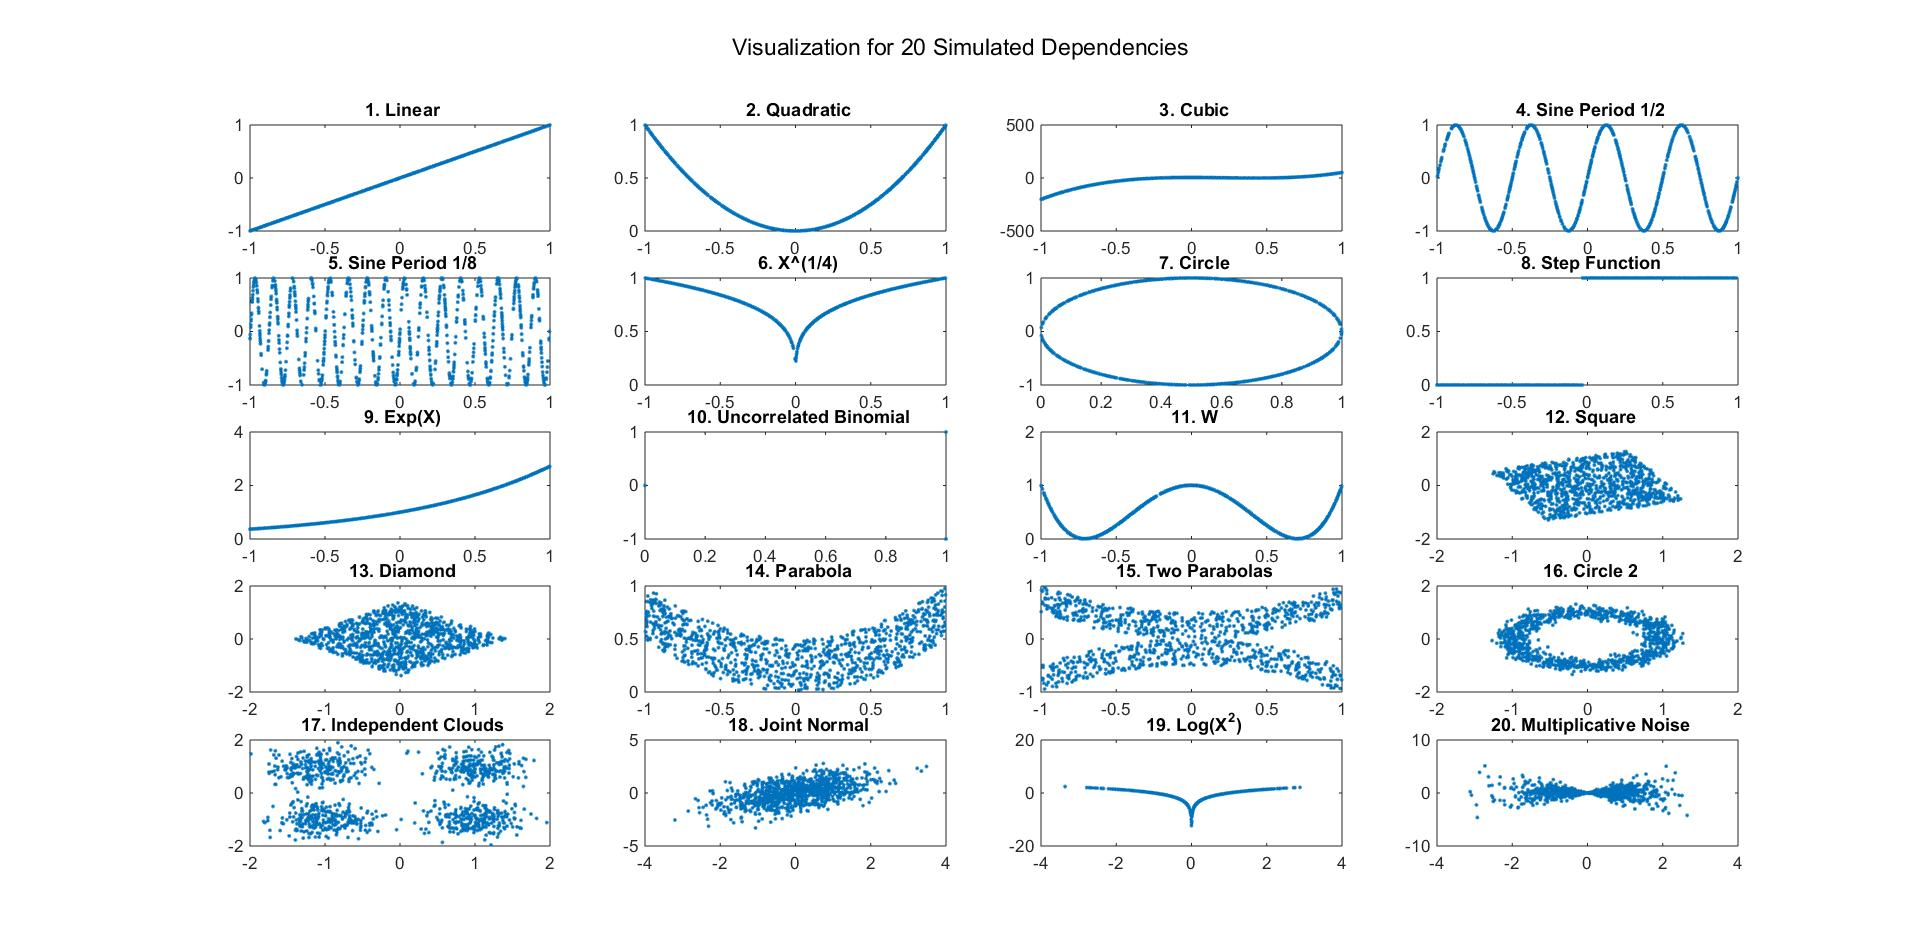
\includegraphics[width=1.0\textwidth]{Fig0}
}
\caption{Visualization of Each Dependency at dimension $1$ and $n=1000$ with no noise}
\label{fig0}
\end{figure}

We consider two different scenarios for those $20$ distributions: a dimension $1$ scenario with increasing sample size, and an increasing dimension scenario with fixed sample size. For the first scenario, we always set $m_{X}=m_{Y}=1$ and plot the power with respect to increasing sample size, so as to observe how fast the testing power of each method converges to $1$ for various dependencies; for the second scenario, we fix $n=100$ and plot the power with respect to increasing $m_{X}$, so as to determine how robust each method is for increasing dimension of each dependency. 

For either scenario, $\mathcal{X}$ and $\mathcal{Y}$ are generated accordingly, then appropriate level of white noise may be added to $\mathcal{Y}$ depending on the distribution (otherwise certain dependency like perfect linear is too easy), and the sample test statistic can be calculated on the sample data. As described in Section~\ref{main3}, we carry out the independence test to estimate the testing power for $r=10000$ Monte-Carlo replicates at $\alpha=0.05$. The empirical powers are shown in Figure~\ref{figSim1} for both the dimension $1$ and increasing dimension scenarios in two separate panels. 

For the dimension $1$ scenario, one may observe that for dependencies that are close to linear, global and local distance correlation always yield similar testing powers, which are better than HHG and Mantel; for the remaining nonlinear dependencies, HHG is usually much better than global distance correlation and Mantel, while local distance correlation performs similarly or even better than HHG in most cases due to its significant improvement over the respective global version. Note that for all distributions other than the independent clouds, the empirical powers eventually increase to $1$ as the sample size increases, implying that all methods are consistent (the only exception is the Mantel test, whose powers stay low in many nonlinear dependencies); and for the independent relationship, all testing powers should be exactly the type $1$ error level, which approximately holds for the empirical testing powers. 

For the increasing dimension scenario, local modified distance correlation significantly surpasses all other methods: for dependencies that are close to linear, the powers of both global and local modified distance correlation deteriorate much slower than others; and for the remaining nonlinear dependencies, local modified distance correlation is much better than all other methods including the global modified distance correlation or the local original distance correlation, due to its capability to better handle non-linearity and high-dimensionality at the same time. Note that a quarter of the distributions (e.g. sine period, square, diamond) cannot be detected by any method at dimension higher than $1$, since all testing powers quickly degrade to around $\alpha$.

To intuitively summarize the simulation performance of each method in all settings, we apply the performance profiles introduced by \cite{DolanMore2002} to the testing powers, which is an evaluation tool to compare different algorithms throughout all given settings. Suppose there are $S$ methods and $T$ different settings, and we denote the respective powers as $\beta_{s}^{t}$ for $s=1,\ldots,S$ and $t=1,\ldots,T$. Then the performance profile for each method is defined as follows:
\begin{align*}
profile_{s}(x) &= \frac{1}{T} \sum_{t=1}^{T} I((\beta_{*}^{t}-\beta_{s}^{t}) \leq x)
\end{align*}
where $x \in [0,1]$ and $\beta_{*}^{t} =\max_{s} \beta_{s}^{t}$ denotes the best testing power in the $t$th setting. Namely $x$ stands for the difference with respect to the best power, and the performance profile of each method equals the proportion of simulations that the method is worse than the best method by no more than $x$. For example, at $x=0.1$, local modified distance correlation has a performance profile of $0.75$ if and only if there are $15$ out of $20$ simulations that local modified distance correlation is worse than the best method by no more than $0.1$ in testing power; the performance profile at $x=0$ stands for the proportion of simulations that the method has the best power; and the performance profile always increases to $1$ at $x=1$. The best method should have a similar or higher curve than others; and we also plot the area under curve for each profile curve in the legend, which is a numerical way of viewing the advantage of each method.

In Figure~\ref{figSim3} we show the performance profiles at fixed dimension and sample size that are determined by a threshold, for both the dimension $1$ and increasing dimension scenarios: for the dimension $1$ scenario, the dimension is always fixed at $1$, so the sample size is determined by the first sample size that any method has a power of $0.8$ (otherwise pick the largest sample size); and for the increasing dimension scenario, the sample size is already fixed at $100$, so we determine the dimension choice by the first dimension that any method has a power that is lower than $0.5$ (otherwise pick the smallest dimension). The threshold choices are arbitrary, and additional plots of varying thresholds are provided in the appendix.

We can clearly see from Figure~\ref{figSim3} that local distance correlation is indeed the most reliable method in finite-sample testing, in accordance with the individual power plots in Figure~\ref{figSim1}: for the dimension $1$ scenario the performance profiles of local original distance correlation and local modified distance correlation are similar to each other and much better than others; and for the increasing dimension scenario local modified distance correlation is significantly better than all other methods. Note that HHG is slightly better than global distance correlation in the performance profiles, because there are more nonlinear distributions than linear in the $20$ dependencies, and HHG has a larger advantage for nonlinear dependency than its disadvantage in linear dependency when compared to global distance correlation; and the Mantel test has the lowest performance profile in both scenarios.

\begin{figure}[htbp]
\subfloat[]{
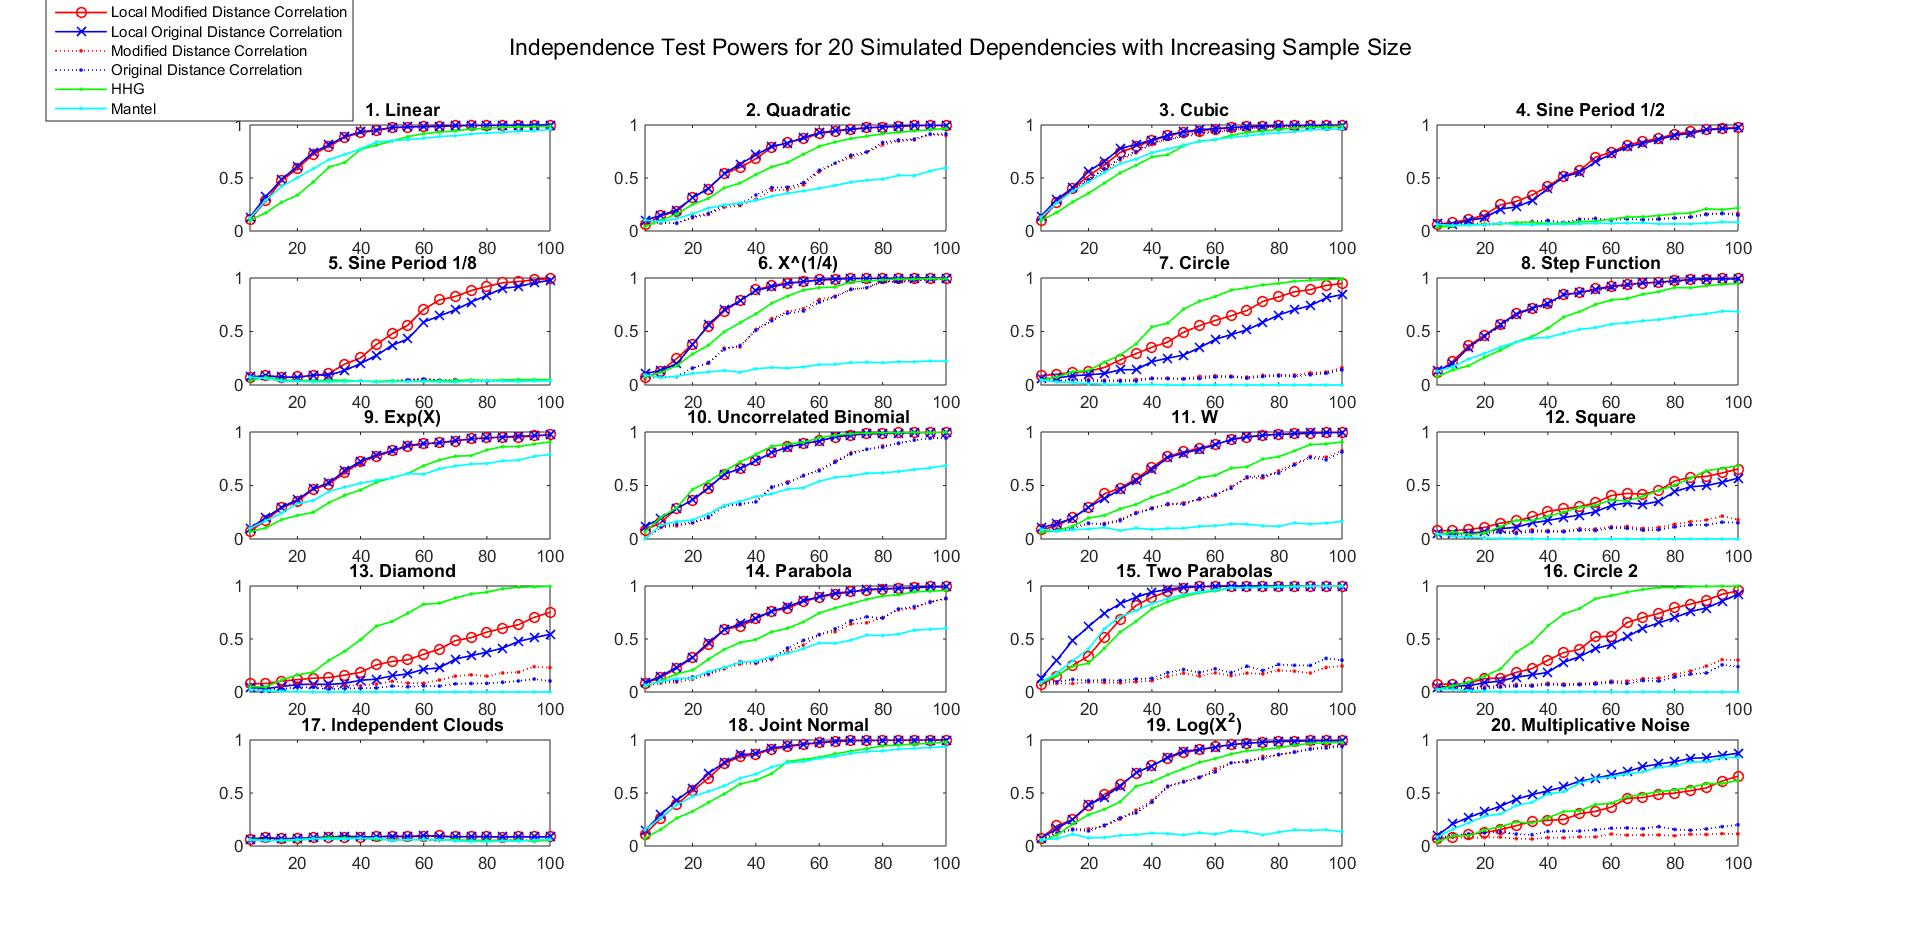
\includegraphics[width=1.0\textwidth]{Fig1}
}
\hfil
\subfloat[]{
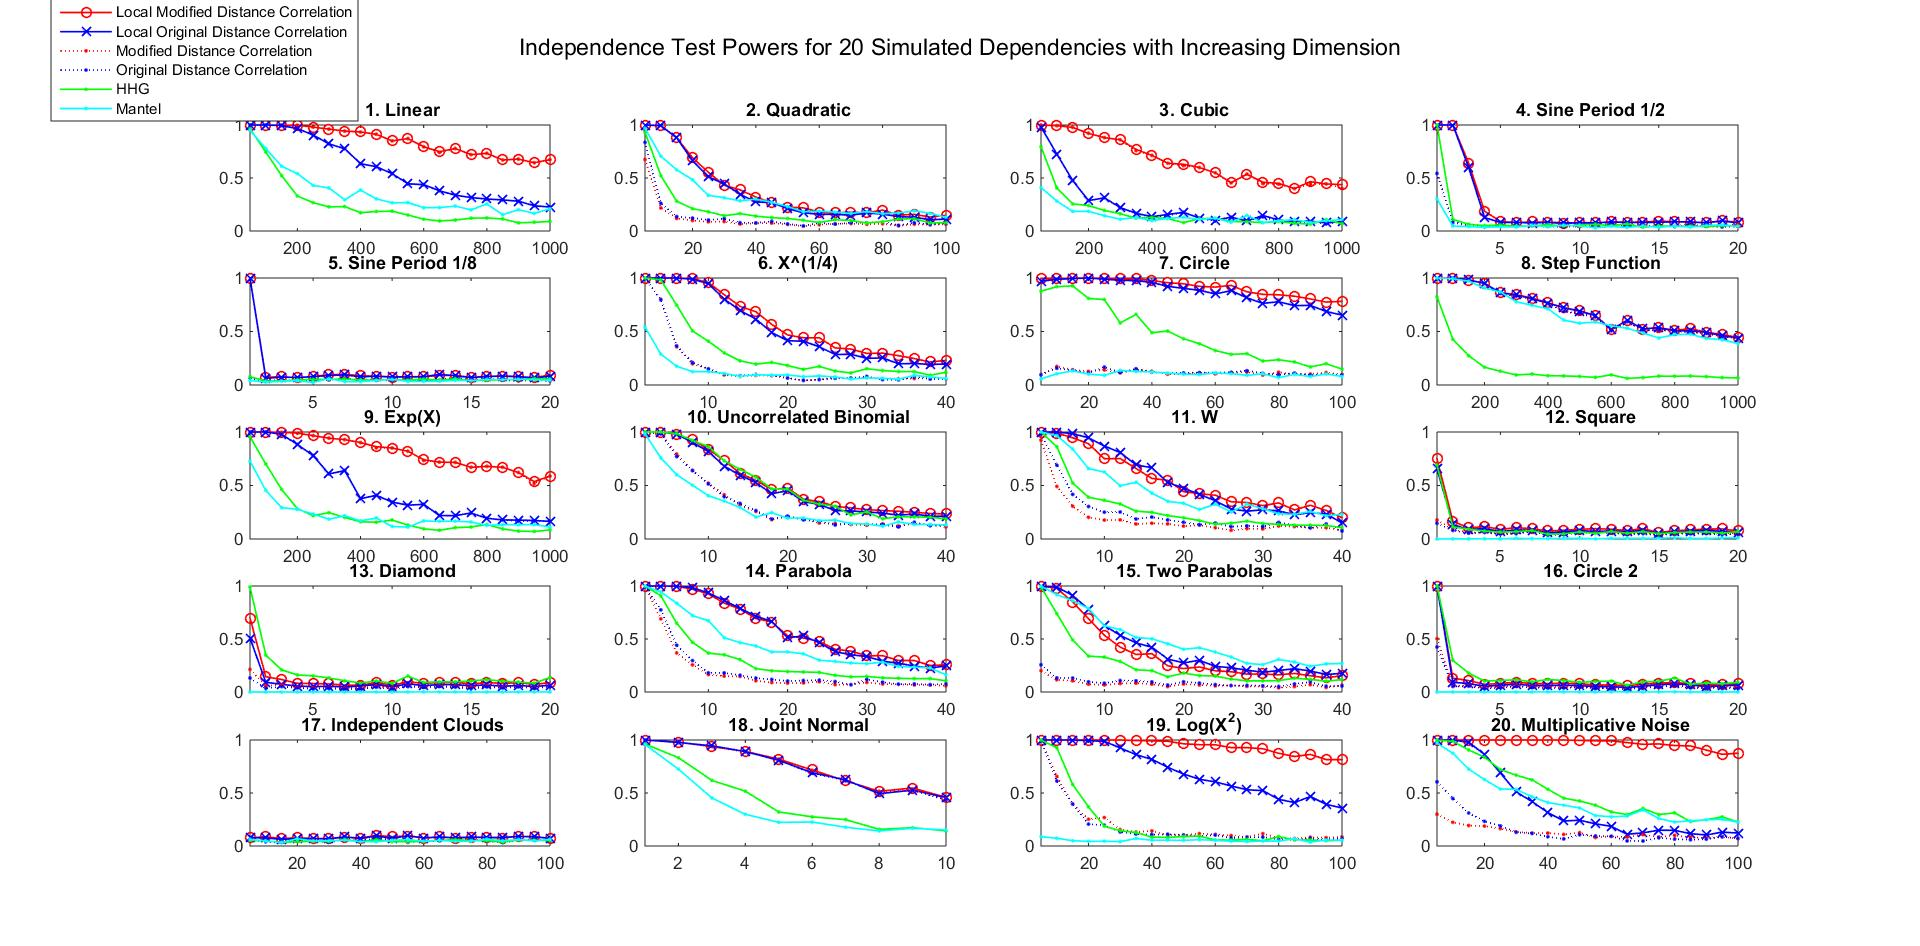
\includegraphics[width=1.0\textwidth]{Fig5}
}
\caption{Testing Power for 20 Simulations of Increasing Sample Size and Dimension}
\label{figSim1}
\end{figure}

\begin{comment}
\begin{figure}[htbp]
\subfloat[]{
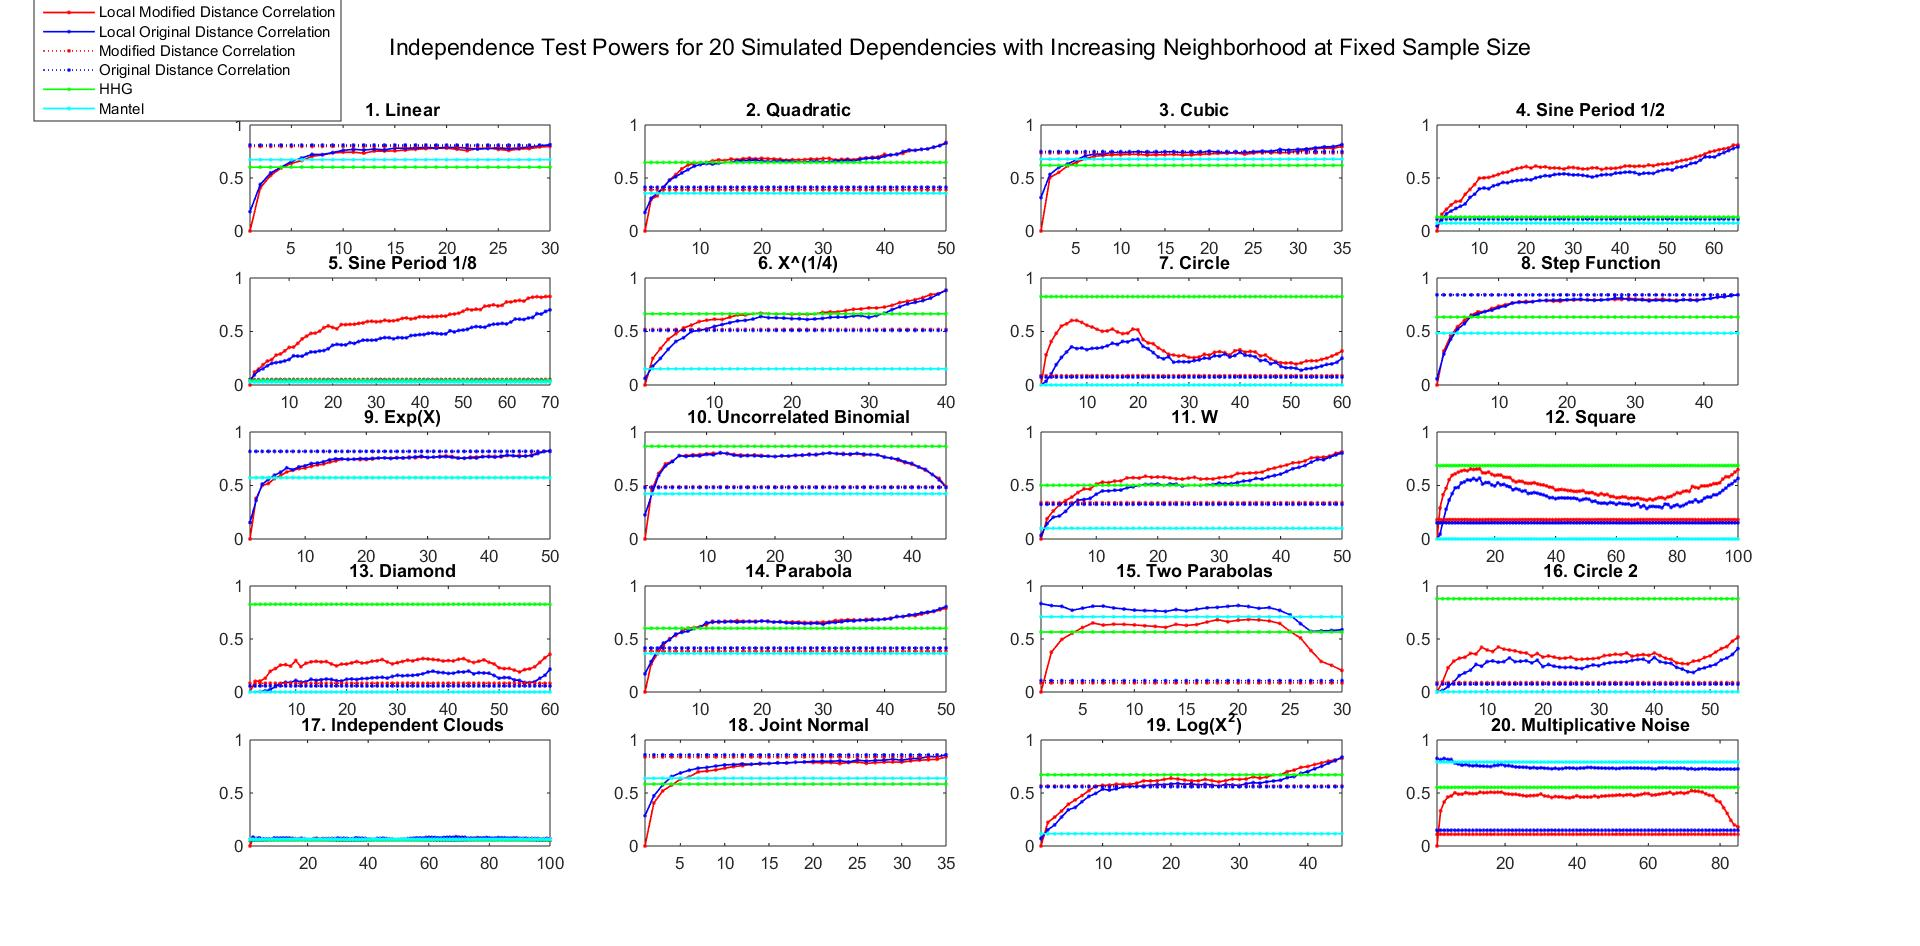
\includegraphics[width=1.0\textwidth]{Fig2}
}
\hfil
\subfloat[]{
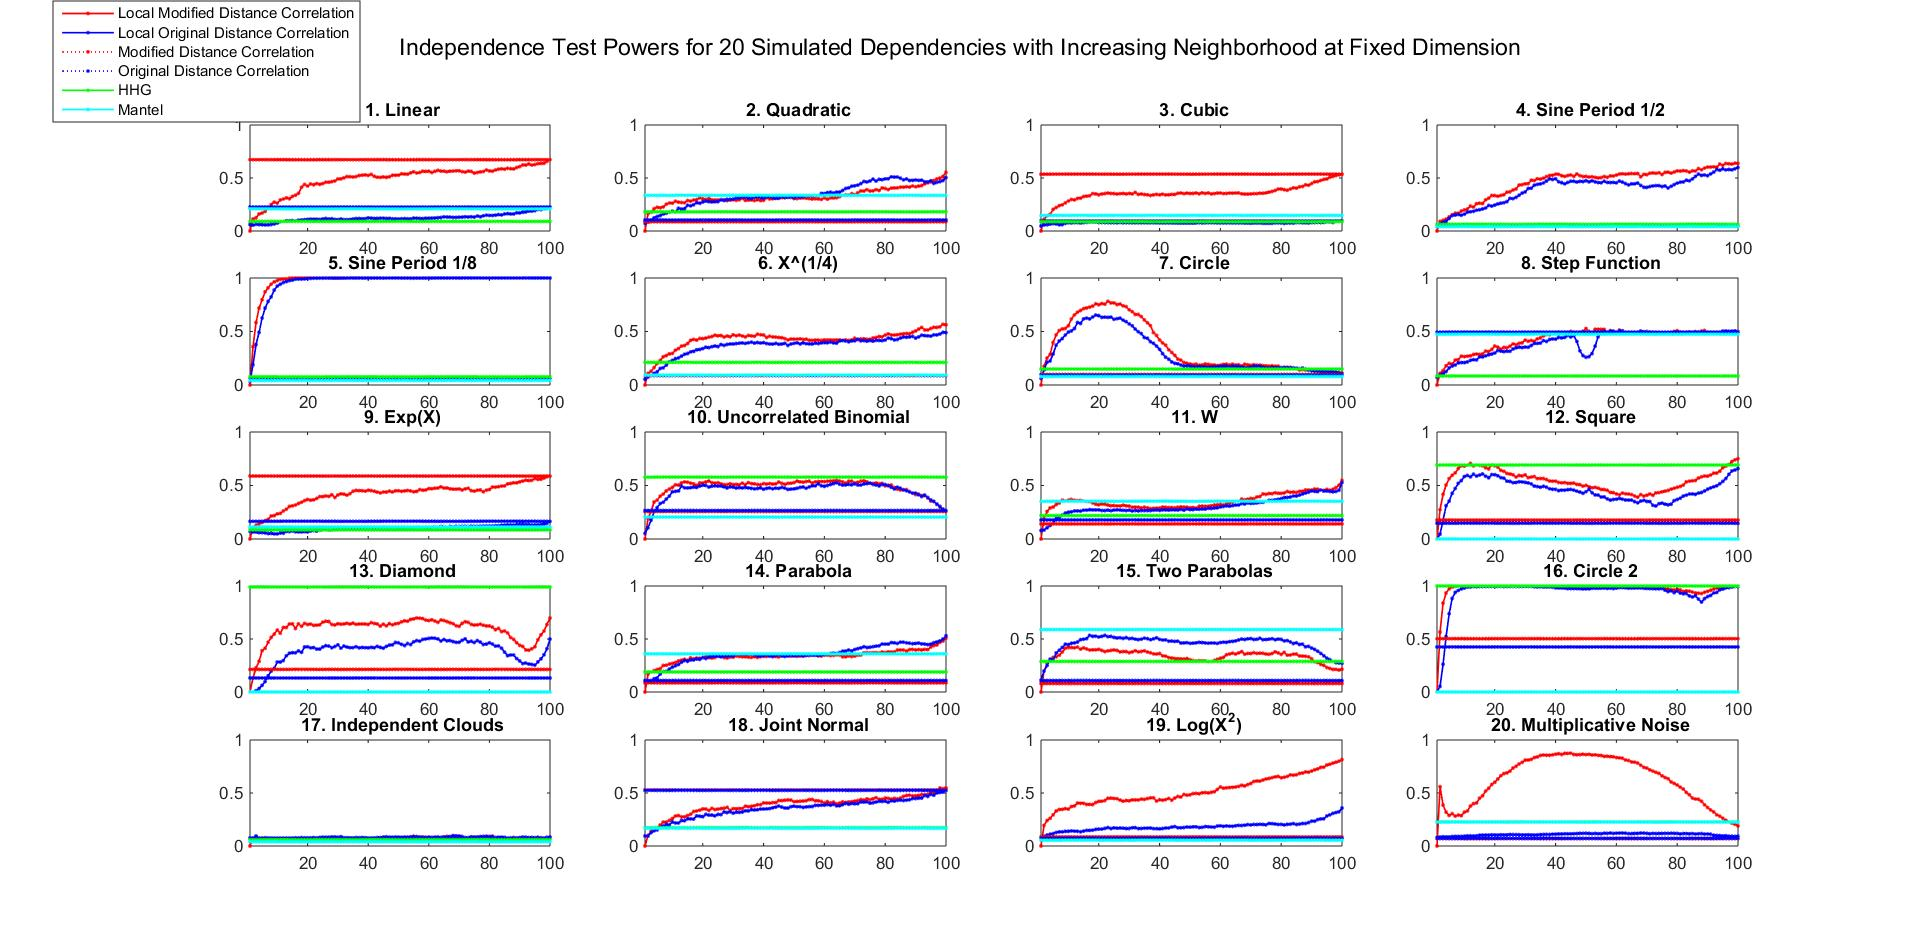
\includegraphics[width=1.0\textwidth]{Fig6}
}
\caption{Testing Power for 20 Simulations of Increasing Neighborhood at Fixed Sample Size and Dimension}
\label{figSim2}
\end{figure}
\end{comment}

\begin{figure}[htbp]
\subfloat[]{
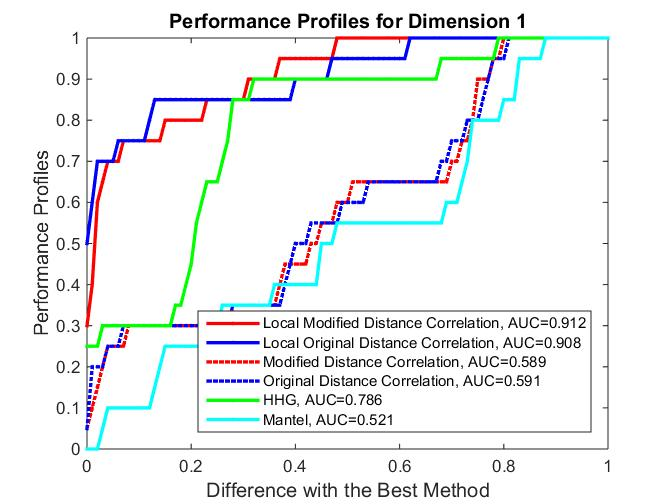
\includegraphics[width=0.5\textwidth]{Fig3}
}
\hfil
\subfloat[]{
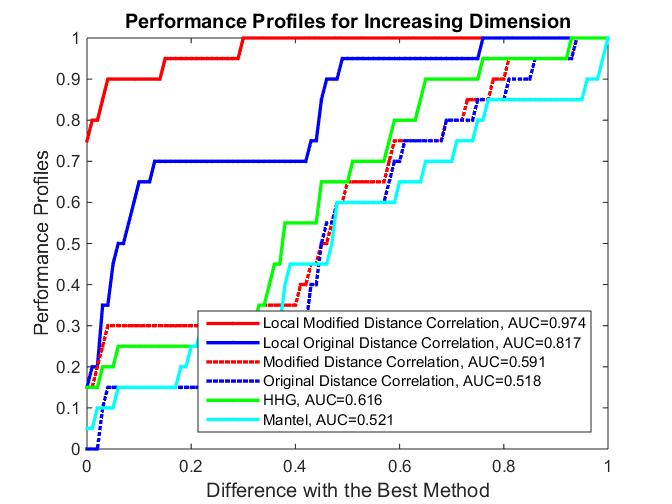
\includegraphics[width=0.5\textwidth]{Fig7}
}
\caption{Performance Profiles on Testing Powers for 20 Simulations}
\label{figSim3}
\end{figure}

\subsection{Real Data}
\label{numer2}
Here we apply the local distance correlation to test independence between brain features and personal characteristics from two different experiments, for which the data sets are relatively small in sample size due to the expensive data collection process. 

The first experiment is to detect the relationship between the brain connectome and personality from \cite{AdelsteinEtAl2011}. The sample size is $n=42$, and each person has a $5$ dimensional personality data based on questionnaires and the five-factor personality model. Then the brain activity of each person is measured by fMRI for $197$ brain regions and $194$ time steps. Thus the brain connectome feature is high-dimensional while the personality data is low-dimensional. There seems to exist certain correlation between the brain activity and personality as experimentally shown in \cite{AdelsteinEtAl2011}, but whether the dependency can be detected from the raw data is the question here.

To apply distance correlation and HHG, first we need to find two distance measures for the different data sources: for the personality data, the distance matrix $A$ is formed by the Euclidean distance directly; for the connectome data, we run a spectrum analysis for each region, bandpass and normalize it, then calculate the Kullback-Leibler divergence among regions and use the normalized Hellinger distance as the distance matrix $B$. Once the distance matrices $A$ and $B$ are obtained, we apply the permutation test in Section~\ref{main3} for $r=10000$ random permutations, and show the log scaled p-value in the first plot of Figure~\ref{figReal}: The x-axis is the neighborhood choice from $1$ to $n$, and the y-axis is the log scaled empirical p-value of $\min_{l} \{\mbox{p-value}(dCorr_{kl})\}$ for local distance correlation, otherwise straight lines. 

The p-value by local modified distance correlation is $0.0276$ achieved at $k=11, l=5$; the p-value by local original distance correlation is $0.3833$ achieved at $k=11, l=35$; original distance correlation has a p-value of 0.6745; modified distance correlation has a p-value of 0.3759; HHG has a p-value of $0.0576$; and the Mantel test has a p-value of $0.9886$. Therefore only local distance correlation has significant (less than $0.05$) p-value, although HHG is quite close to significant as well.

\begin{figure}[htbp]
\centering
\subfloat[]{
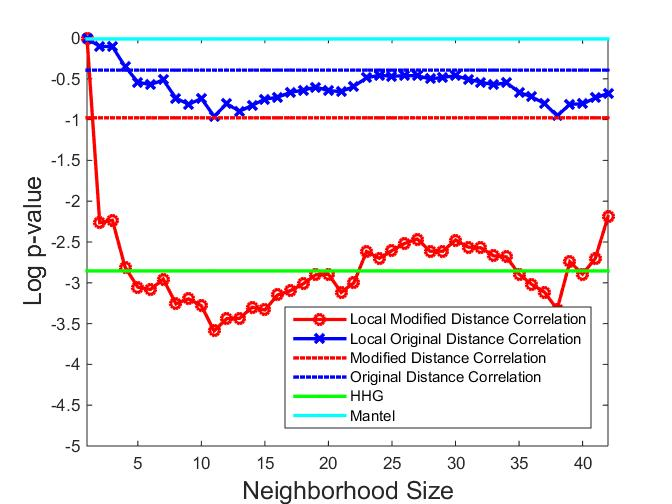
\includegraphics[width=0.5\textwidth]{FigReal1Log}
}
\hfil
\centering
\subfloat[]{
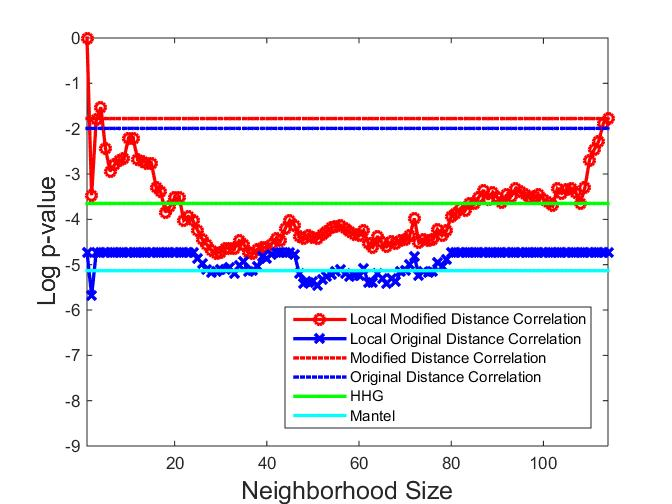
\includegraphics[width=0.5\textwidth]{FigReal2Log}
}
\hfil
\centering
\subfloat[]{
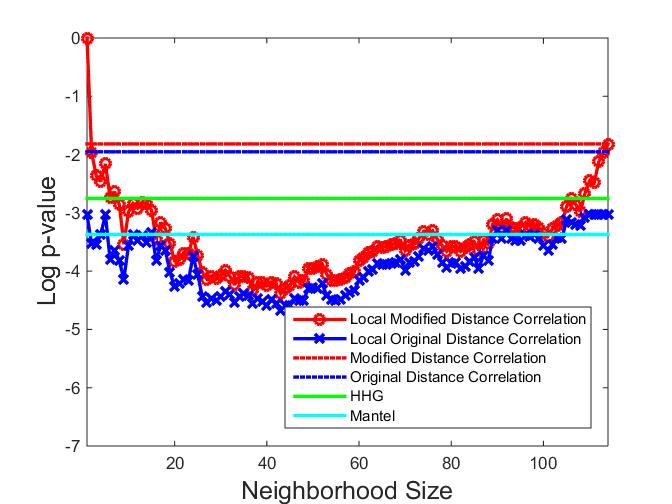
\includegraphics[width=0.5\textwidth]{FigReal3Log}
}
\caption{P-value of Real Data Testing}
\label{figReal}
\end{figure}

Next we carry out the same testing procedure on another experiment regarding brain hippocampus shape and major depressive disorder. There are $n=114$ subjects, and the brain images of each person are obtained by very high resolution MRI scans on the hippocampus; and we also have available a categorical vector containing the disease information, including clinically depressed subject, high-risk subject, and non-affected subject. 

The brain data is transformed into two dissimilarity matrices $LML$ and $LMR$, representing the left and right hippocampus data based on landmark matching (see \cite{ParkEtAl2011} for more details on data processing); and the label vector is transformed into a binary dissimilarity matrix $D$, where $D(i,j)=0$ if and only if the $i$th subject has a different label from the $j$th subject.

There has been evidences that relate major depressive disorder to the hippocampus shape in \cite{ParkEtAl2011} and \cite{PosenerEtAl2003}, and we would like to test the significance of such relationship in the data. In the second plot of Figure~\ref{figReal}, we show the log scaled p-value of permutation test between $LML$ and $D$, and in the third plot of Figure~\ref{figReal} we show the log scaled p-value for testing between $LMR$ and $D$. 

In both plots, local distance correlation yields lower p-values than its global version and HHG. For testing between $LML$ and $D$, the actual p-value of local modified distance correlation is $0.0086$ achieved at $k=37,l=23$, $0.0034$ for local original distance correlation achieved at $k=2,l=5$, $0.1690$ and $0.1362$ for global modified and local distance correlation, $0.0260$ for HHG, and $0.0059$ for Mantel. For testing between $LMR$ and $D$, the actual p-value of local modified distance correlation is $0.0124$ achieved at $k=43,l=114$, $0.0094$ for local original distance correlation achieved at $k=43,l=114$ too, $0.1624$ and $0.1419$ for global modified and original distance correlation, $0.0638$ for HHG, and $0.0344$ for Mantel. Again the p-values of local distance correlation are very significant, although HHG and the Mantel test have significant p-values as well.

Note that the p-value is always $0$ for any testing statistic when testing independence between $LML$ and $LMR$, implying strong linear dependency between the left and right brain.

\section{Conclusion}
\label{conclu}
In short, we propose the local distance correlation to test independence between data sets, which has been shown to be perform well for testing independence on data of small sample size, high-dimensionality, linearity or non-linearity. It not only enjoys theoretical guarantee such as being consistent in testing independence, but also exhibits superior numerical performances in a comprehensive simulation setting and real data experiments, comparing to other popular methods.

\section*{Acknowledgment}
\addcontentsline{toc}{section}{Acknowledgment}
This work was partially supported by National Security Science and Engineering Faculty Fellowship (NSSEFF),
 Johns Hopkins University Human Language Technology Center of Excellence (JHU HLT COE), and the
 XDATA program of the Defense Advanced Research Projects Agency (DARPA) administered through Air Force Research Laboratory contract FA8750-12-2-0303.


\bibliographystyle{chicago}
\bibliography{references}

\end{document}